\documentclass[a4paper,12pt]{article}

%%% Работа с русским языком

\usepackage{cmap}					% поиск в PDF
\usepackage{mathtext} 				% русские буквы в формулах
\usepackage[T2A]{fontenc}			% кодировка
\usepackage[utf8]{inputenc}			% кодировка исходного текста
\usepackage[english,russian]{babel}	% локализация и переносы
\usepackage{indentfirst}            % красная строка в первом абзаце
\usepackage[unicode]{hyperref}
\usepackage{epigraph}
\frenchspacing                      % равные пробелы между словами и предложениями

%%% Дополнительная работа с математикой
\usepackage{amsmath,amsfonts,amssymb,amsthm,mathtools} % пакеты AMS
\usepackage{bbm} % Blackboard bold для цифр
\usepackage{icomma}                                    % "Умная" запятая

\renewcommand{\phi}{\ensuremath{\varphi}}
\renewcommand{\kappa}{\ensuremath{\varkappa}}
\renewcommand{\le}{\ensuremath{\leqslant}}
\renewcommand{\leq}{\ensuremath{\leqslant}}
\renewcommand{\ge}{\ensuremath{\geqslant}}
\renewcommand{\geq}{\ensuremath{\geqslant}}
\renewcommand{\emptyset}{\ensuremath{\varnothing}}

\newcommand{\cl}{\text{cl }}
\newcommand{\setint}{\text{int }}

\theoremstyle{plain}
\newtheorem{theorem}{Теорема}[section]
\newtheorem{lemma}{Лемма}[section]
\newtheorem{proposition}{Утверждение}[section]
\newtheorem*{corollary}{Следствие}
\newtheorem*{exercise}{Упражнение}

\theoremstyle{definition}
\newtheorem{definition}{Определение}[section]
\newtheorem*{note}{Замечание}
\newtheorem*{reminder}{Напоминание}
\newtheorem*{example}{Пример}
\newtheorem*{tasks}{Вопросы и задачи}

\theoremstyle{remark}
\newtheorem*{solution}{Решение}

%%% Оформление страницы
\usepackage{extsizes}     % Возможность сделать 14-й шрифт
\usepackage{geometry}     % Простой способ задавать поля
\usepackage{setspace}     % Интерлиньяж
\usepackage{enumitem}     % Настройка окружений itemize и enumerate
\setlist{leftmargin=25pt} % Отступы в itemize и enumerate

\geometry{top=25mm}    % Поля сверху страницы
\geometry{bottom=30mm} % Поля снизу страницы
\geometry{left=20mm}   % Поля слева страницы
\geometry{right=20mm}  % Поля справа страницы

\begin{document}
\tableofcontents
\newpage

\section{Теорема Римана об осцилляции}

\begin{definition}
	Точка $x$ называется \textbf{точкой прикосновения} множества $S$, если любая окресность $x$ содержит хотя бы одну точку множества $S$.
\end{definition}

\begin{definition}
	Множество всех точек прикочновения $S$ называется \textbf{замыканием} $S$.
\end{definition}

\begin{definition}
	\textbf{Носителем} функции $f(x)$ называется замыкание множества тех $x$, для которых $f(x) \neq 0$. (supp $f$) Функции с ограниченным носителем называются \textbf{финитными}.
\end{definition}

\begin{definition}
	Множество $D$ называется всюду плотным в множестве $G$, если
	\[\overline{D} = G\]
\end{definition}

\begin{proposition}
	$L_1(\mathbb{R})$ -- линейное нормированное пространство.
	\[\|f\|_1 = \int_\mathbb{R} |f(x)| d\mu(x)\]
\end{proposition}

\begin{lemma}
	\label{C_IN_PLOTNI}

	Множество непрерывных финитных функций всюду плотно в $L_1(\mathbb{R})$.
\end{lemma}

\begin{proof}
	Заменим $\mathbb{R}$ на $[a,\,b]$. То есть докажем, что множество непрерывных на $[a,\,b]$ функций всюду плотно в $L_1[a,\,b]$.

	\begin{itemize}
		\item Любая суммируемая функция представима в виде разности двух неотрицательных суммируемых функций, поэтому достатончо доказать утверждение для
			  неотрицательных суммируемых функций.
		\item Так как интеграл неотрицательной суммируемой функции слабо отличается от интеграла её срезки $f_{[N]}(x)$ при достаточно больших $N$, то
		      достаточно доказать утверждение для ограниченных неотрицательных суммиремых функций.
		\item Докажем для ограниченных неотрицательных. По теореме о представлении ограниченной измеримой функции пределом последовательности ступенчатых
		      \[\exists \{h_n\}:\: h_n \uparrow f\]
		      Теорема Леви гарантирует, что
		      \[\int_a^b h_n(x)d\mu(x) \to \int_a^b f(x)d\mu(x)\]
		      Значит
		      \begin{align*}
			      \int_a^b |f(x) - h_n(x)|d\mu(x) = \int_a^b (f(x) - h_n(x))d\mu(x) \stackrel{n \to +\infty}{\to} 0
		      \end{align*}
		      То есть нам достаточно доказать, что любую ступенчатую можно приблизить непрерывной:
		      \[h_n(x) = \sum_{k = 1}^N c_k \mathbb{I}_{E_k}(x)\]
		      В силу того, что $\forall k:\: E_k$ -- измеримое, то
		      \[\forall \varepsilon > 0:\: \exists \text{элементарное } M_\varepsilon:\: \mu(E_k \triangle M_\varepsilon) < \varepsilon \]
		      Значит
		      \[\int_a^b |\mathbb{I}_{E_k}(x) - \mathbb{I}_{M_\varepsilon}(x)|d\mu(x) = \int_a^b \mathbb{I}_{E \triangle M_\varepsilon}(x)d\mu(x) = \mu(E \triangle M_\varepsilon) < \varepsilon\]
		      Нам осталось научиться приблизить индикатор интервала непрерывными функциями (так как элементарное множество представимо объединением интервалов), а это сделать очень просто, используя непрерывную функцию $\phi(x)$, которая выглядит вот так:
		      \begin{figure}[h]
			      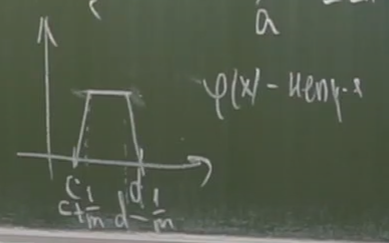
\includegraphics[scale=0.5]{img/phi_graph.png}
			      \caption{Один из способов ввода функции $\phi$}
		      \end{figure}
		      Тогда
		      \[\int_a^b |\mathbb{I}_{(c,\,d)}(x) - \phi(x)|d\mu(x) = \frac{2}{m} < \varepsilon\]
	\end{itemize}

	Возвращаемся к общему случаю: пусть $f \in L_1(\mathbb{R})$.

	\[\exists N \in \mathbb{N}\: \int_{\mathbb{R} \setminus [-N,\,N]}|f(x)|d\mu(x) < \frac{\varepsilon}{3}\]
	По доказанному выше:
	\[f|_{[-N,\,N]} :\: \forall \varepsilon > 0 \:\exists g \in C[-N,\,N] \: \|f|_{[-N,\,N]} - g\|_{L_1[-N,\,N]} < \frac{\varepsilon}{3}\]
	Далее мы можем продлить $g$ на всю прямую линейных образом (аналогично введению функции $\phi$ из рассуждений выше), так, чтобы
	\[\int_{\mathbb{R}\setminus [-N,\,N]} |g(x)|d\mu(x) < \frac{\varepsilon}{3}\]
	Тогда
	\[\int_\mathbb{R} |f(x) - g(x)|d\mu(x) \leq \int_{-N}^N |f(x) - g(x)|d\mu(x) + \int_{\mathbb{R} \setminus [-N,\,N]} (|f(x)| + |g(x)|) d\mu(x) < \varepsilon\]
\end{proof}

\begin{lemma}
	\label{CONT_MODUL}

	Каждая суммируемая на $\mathbb{R}$ функция $f(x)$ непрерывна в среднем относительно сдвига, то есть
	\[\lim_{t \to 0} \int_\mathbb{R} |f(x + t) - f(x)| d\mu(x) = 0\]
\end{lemma}

\begin{proof}
	Докажем, что для $f \in L_1[a,\,b]$:
	\[\lim_{\delta \to +0} \sup_{0 \leq h \leq \delta} \int_a^{b - h} |f(x + h) - f(x)|d\mu(x) = 0\]
	По предыдущей лемме:
	\[\forall \varepsilon > 0 \: \exists g \in C[a,\,b]:\: \int_a^b |f(x) - g(x)|d\mu(x) < \frac{\varepsilon}{3}\]
	$g$ -- непрерывная на $[a,\,b] \Rightarrow$ по теореме Кантора:
	\[\forall \varepsilon > 0 \: \exists \delta > 0 \: \forall x,\,y \in [a,\,b],\, |x - y| < \delta :\: |g(x) - g(y)| < \frac{\varepsilon}{3(b - a)}\]
	Тогда $\forall h \: 0 \leq h \leq \delta$:
	\begin{align*}
		\int_a^{b - h}|f(x + h) - f(x)|d\mu(x) \leq \int_a^{b - h} |f(x + h) - g(x + h)|d\mu(x) + \int_a^{b - h}|f(x) - g(x)|d\mu(x) + \\
		+ \int_a^{b - h}|g(x + h) - g(x)|d\mu(x) < \varepsilon
	\end{align*}
	Так как $f$ суммируема на $\mathbb{R}$, то $\exists N \in \mathbb{N}$:
	\[\int_{\mathbb{R} \setminus [-N,\,N]}|f(x)|d\mu(x) < \frac{\varepsilon}{3}\]
	Тогда выберем $[a,\,b] := [-N - 1,\,N + 1]$ и введём $g := f\mathbb{I}_{[-N,\,N]} \in L_1[a,\,b]$. Применим к этой функции доказанное выше равенство:
	\[\exists \delta \in (0,\,1) \: \forall h,\, 0 \leq h \leq \delta :\: \int_a^{b - h}|g(x + h) - g(x)|d\mu(x) < \frac{\varepsilon}{3}\]
	Теперь возьмём $\forall t,\, |t| < \delta$:
	\[
		\int_\mathbb{R}|f(x + t) - f(x)|d\mu(x) = \int\limits_{\{x,\,x+t\}\subseteq[a,\,b]}|f(x+t)-f(x)|d\mu(x) + \int\limits_{\{x,\,x+y\}\not\subseteq[a,\,b]}|f(x+t)-f(x)|d\mu(x) < \varepsilon
	\]
\end{proof}

\begin{theorem}
	Римана об осцилляции.

	Если $f \in L_1(I)$, где $I$ -- конечный или бесконечный промежуток, то
	\[\lim_{\lambda \to \infty} \int_I f(x)\cos(\lambda x) d \mu(x) = \lim_{\lambda \to \infty} \int_I f(x) \sin (\lambda x) d\mu(x) = 0\]
\end{theorem}

\begin{proof}
	\begin{align*}
		\int_I f(x) \cos(\lambda x) d\mu(x) \stackrel{x = t + \frac{\pi}{\lambda}}{=} - \int_{I - \frac{\pi}{\lambda}} f\left( t + \frac{\pi}{\lambda} \right) \cos(\lambda t) d \mu(t) = \\
		-\frac{1}{2} \int_I \left(f\left(t + \frac{\pi}{\lambda}\right) - f(t) \right)\cos(\lambda t) d\mu(t) - \frac{1}{2} \int_{(I - \frac{\pi}{\lambda}) \triangle I} f\left(t + \frac{\pi}{\lambda}\right) \cos(\lambda t) d \mu(t)
	\end{align*}
	Заметим, что
	\begin{align*}
		\left|\int_{(I - \frac{\pi}{\lambda}) \setminus I} f\left(t + \frac{\pi}{\lambda}\right) \cos(\lambda t) d \mu(t)\right| \leq \int_{(I - \frac{\pi}{\lambda}) \triangle I} \left|f\left(t + \frac{\pi}{\lambda}\right)\right| d\mu(t) = \\
		= \int_{I \triangle (I + \frac{\pi}{\lambda})} |f(x)|d\mu(t) \stackrel{\lambda \to \infty}{\to} 0
	\end{align*}
	Последнее заключение следует из того, что $\mu\left(I \triangle (I + \frac{\pi}{\lambda})\right) \stackrel{\lambda \to \infty}{\to} 0$

	Также очевидно, что
	\begin{align*}
		\left|\int_I \left(f\left(t + \frac{\pi}{\lambda}\right) - f(t) \right)\cos(\lambda t) d\mu(t)\right| \leq \int_I \left|f\left(t + \frac{\pi}{\lambda}\right) - f(t)\right|d\mu(t) \stackrel{\text{по пред. Лемме}}{\to} 0
	\end{align*}
\end{proof}

\section{Представление частичной суммы ряда Фурье интегралом с ядром Дирихле. Принцип локализации.}
\begin{definition}
	$f \in L_{2\pi} \Leftrightarrow f \in L_1[-\pi,\,\pi]$ и $2\pi$ периодическая.
\end{definition}

\begin{definition}
	Ядром Дирихле $D_n(u)$ называется выражение
	\[D_n(u) = \frac{1}{2} + \sum_{k = 1}^n \cos(ku) = \frac{\sin (n + \frac{1}{2})u}{2\sin(\frac{u}{2})}\]
\end{definition}

\begin{proof}
	\begin{align*}
		D_n(u) = \frac{1}{2} + \sum_{k = 1}^n \cos(ku) = \frac{1}{2} + \frac{1}{2}\sum_{k = 1}^n (e^{iku} + e^{-iku}) = \frac{1}{2}\sum_{k = -n}^n e^{iku} = \frac{1}{2}e^{-inu}\frac{e^{i(2n + 1)u} - 1}{e^{iu} - 1} = \\
		= \frac{1}{2}e^{-inu}\frac{e^{i(2n + 1)\frac{u}{2}} - e^{-i(2n + 1)\frac{u}{2}}}{e^{i\frac{u}{2}} - e^{-i\frac{u}{2}}}\cdot\frac{e^{i(2n + 1)\frac{u}{2}}}{e^{i\frac{u}{2}}} = \frac{1}{2}\frac{\sin((n + \frac{1}{2})u)}{\sin(\frac{u}{2})}
	\end{align*}
\end{proof}

\begin{lemma}
	О представлении частичной суммы.

	Если $f \in L_{2\pi}$, то $n$-я частичная сумма тригонометрического ряда Фурье
	\[S_n(f,\,x) = \frac{a_0}{2} + \sum_{k = 1}^n a_k \cos(kx) + b_k\sin(kx)\]
	может быть представлена следующим образом:
	\[S_n(f,\,x) = \frac{1}{\pi}\int_{-\pi}^\pi f(t)D_n(x - t)d\mu(t) = \frac{1}{\pi}\int_{-\pi}^\pi f(x + u)D_n(u)d\mu(u)\]
\end{lemma}

\begin{proof}
	Подставим в $S_n$ формулы для $a_k,\, b_k$:
	\begin{align*}
		S_n(f,\,x) = \frac{1}{\pi}\int_{-\pi}^\pi f(t) \left(\frac{1}{2} + \sum_{k = 1}^n (\cos(kx)\cos(kt) + \sin(kx)\sin(kt))\right)d\mu(t) = \\
		= \frac{1}{\pi}\int_{-\pi}^\pi f(t)D_n(x-t)d\mu(t)
	\end{align*}
	Первая формула доказана, вторая доказывается очевидно заменой $t = x + u$, а также используя тот факт, что интеграл по любому отрезку длины $T$, $T$-периодичной функции одинаков.
\end{proof}

\begin{lemma}
	Пусть $f \in L_{2\pi}$, $g$ -- измеримая, $2\pi$-периодическая, ограниченная функция. Тогда коэффициенты Фурье функции $\chi(t) = f(x + t)g(t)$ стремятся к нулю при $n \to +\infty$ равномерно по $x$.
\end{lemma}

\begin{proof}
	$g$ -- ограниченная $\Rightarrow \exists M:\: \forall u \: |g(u)| \leq M$.

	$f$ -- измеримая $\Rightarrow$ по (\ref{C_IN_PLOTNI}) мы можем её представить, как $f = f_1 + f_2$, причём $f_1 \in C[-\pi,\,\pi]$, а $\int_{-\pi}^{\pi} |f_2(t)|d\mu(t) < \frac{\varepsilon}{4M}$.

	$f_1$ -- непрерывная на компакте $[-\pi,\,\pi] \Rightarrow \exists B \: \forall u:\: |f_1(u)| \leq B$.

	Введём функцию, которая называется интегральный модуль непрерывности функции $F$:
	\[\omega_1(\delta,\,F) := \sup_{0 \leq h \leq \delta} \int_{-\pi}^\pi |F(t + h) - F(t)|d\mu(t)\]
	Рассмотрим $a_n$ для функции $\chi$:
	\begin{align*}
		a_n(\chi) = \frac{1}{\pi} \int_{-\pi}^\pi \chi(t)\cos(nt)d\mu(t) = \stackrel{t = u + \frac{\pi}{n}}{=} \frac{-1}{\pi}\int_{-\pi}^\pi \chi\left(u + \frac{\pi}{n}\right)\cos(nu)d\mu(u) = \\
		= \frac{-1}{2\pi}\int_{-\pi}^\pi \left[\chi\left(t + \frac{\pi}{n}\right) - \chi(t)\right]\cos(nt)d\mu(t) \Rightarrow\\
		|a_n(\chi)| \leq \frac{1}{2\pi}\omega_1\left(\frac{\pi}{n},\, \chi\right)
	\end{align*}
	Аналогично получим неравенство для $b_n(\chi)$:
	\[|b_n(\chi)| \leq \frac{1}{2\pi}\omega_1\left(\frac{\pi}{n},\,\chi\right)\]
	То есть мы свели доказательство к доказательству факта, что $\lim_{n \to +\infty}\omega_1(\frac{\pi}{n},\,\chi) = 0$ равномерно по $x$:
	\begin{align*}
		\int_{-\pi}^\pi |\chi(t + h) - \chi(t)|d\mu(t) = \int_{-\pi}^\pi |f(x + t + h)g(t + h) - f(x + t)g(t)|d\mu(t) \leq \\
		\leq \int_{-\pi}^\pi |f(x + t + h) - f(x + t)|\cdot |g (t + h)|d\mu(t) + \int_{-\pi}^\pi |f(x + t)|\cdot |g(t + h) - g(t)|d\mu(t) \leq \\
		\leq M \int_{-\pi}^\pi |f(u + h) - f(u)|d\mu(u) +  \int_{-\pi}^\pi |f_1(x + t)|\cdot|g(t + h) - g(t)|d\mu(t) + \frac{\varepsilon}{2} \leq \\
		\leq M \omega_1(\frac{\pi}{n},\, f) + B\omega_1(\frac{\pi}{n},\,g) + \frac{\varepsilon}{2}
	\end{align*}
	Но по (\ref{CONT_MODUL}) мы знаем, что модуль непрерывности стремится к нулю при $\delta \to 0$. Что и требовалось доказать.
\end{proof}

\begin{theorem}
	Принцип локализации.

	Если $f \in L_{2\pi}$ и тождественно равна нулю в некотором интервале $(a,\,b) \subset [-\pi,\,\pi]$, то её тригонометрический ряд Фурье сходится к нулю равномерно на любом отрезке $[a',\,b'] \subset (a,\,b)$.
\end{theorem}

\begin{proof}
	Так как $[a',\,b']$ содержится в $(a,\,b)$, то
	\[\exists \eta > 0 \: \forall x \in [a',\,b'] \: \forall t,\, 0 \leq |t| < \eta :\: x + t \in (a,\,b)\]
	Построим функцию $\lambda(t)$:
	\[
		\lambda(t) = \begin{cases}
			0,\, t \in (-\eta,\,\eta) \\
			1,\, t \in [-\pi,\,\pi]\setminus (-\eta,\,\eta)
		\end{cases}
	\]
	Кроме того, $\lambda$ -- $2\pi$-периодическая.

	Тогда, используя лемму о представлении частичной суммы, получим:
	\[
		S_n(f,\,x) = \frac{1}{\pi}\int_{-\pi}^\pi f(x + t)D_n(t)d\mu(t) = \frac{1}{\pi}\int_{-\pi}^\pi f(x + t)\lambda(t)D_n(t)d\mu(t)
	\]
	Данное соотношение верно, так как когда $t \not\in (-\eta,\,\eta)$, то $\lambda(\eta) = 1$, ничего не меняем. Если же $|t| < \eta$, то $x + t \in (a,\,b)$, где $f = 0$, поэтому получили, что подыинтегральные функции совпадают везде на $[-\pi,\,\pi]$.

	Продолжим раскрытия данной формулы, используя тригонометрические соотношения для ядра Дирихле:
	\begin{align*}
		S_n(f,\,x) = \frac{1}{\pi}\int_{-\pi}^\pi f(x + t)\lambda(t)\ctg(\frac{t}{2})\sin(nt)d\mu(t) + \frac{1}{2\pi}\int_{-\pi}^\pi f(x+t)\lambda(t)\cos(nt)d\mu(t)
	\end{align*}
	Взяв в качестве $g$ из предыдущей леммы для первого слагаемого $\lambda(t)\ctg(\frac{t}{2})$ и $\lambda(t)$ для второго, то получим требуемое по этой же лемме.

\end{proof}

\end{document}
